\documentclass[a4paper,twoside]{article}
\usepackage{blindtext}  
\usepackage{geometry}

% Chinese support
\usepackage[UTF8, scheme = plain]{ctex}

% Page margin layout
\geometry{left=2.3cm,right=2cm,top=2.5cm,bottom=2.0cm}


\usepackage{listings}
\usepackage{xcolor}
\usepackage{geometry}
\usepackage{amsmath}
\usepackage{float}
\usepackage{hyperref}

\usepackage{graphics}
\usepackage{graphicx}
\usepackage{epsfig}
\usepackage{float}
\usepackage{caption}
\usepackage{subcaption}

\usepackage{algorithm}
\usepackage[noend]{algpseudocode}

\usepackage{booktabs}
\usepackage{threeparttable}
\usepackage{longtable}
\usepackage{tikz}
\usepackage{multicol}

% cite package, to clean up citations in the main text. Do not remove.
\usepackage{cite}

\usepackage{color,xcolor}

%% The amssymb package provides various useful mathematical symbols
\usepackage{amssymb}
%% The amsthm package provides extended theorem environments
\usepackage{amsthm}
\usepackage{amsfonts}
\usepackage{enumerate}
\usepackage{enumitem}
\usepackage{listings}
\usepackage{minted}


\usepackage{indentfirst}
\setlength{\parindent}{2em} % Make two letter space in the first paragraph
\usepackage{setspace}
\linespread{1.5} % Line spacing setting
\usepackage{siunitx}
\setlength{\parskip}{0.5em} % Paragraph spacing setting

% \usepackage[contents =22920202204622, scale = 10, color = black, angle = 50, opacity = .10]{background}

\renewcommand{\figurename}{图}
\renewcommand{\listingscaption}{代码}
\renewcommand{\tablename}{表格}
\renewcommand{\contentsname}{目录}
\floatname{algorithm}{算法}

\graphicspath{ {images/} }

%%%%%%%%%%%%%
\newcommand{\StudentNumber}{22920202204622}  % Fill your student number here
\newcommand{\StudentName}{熊恪峥}  % Replace your name here
\newcommand{\PaperTitle}{实验(二)流水线与流水线中的冲突}  % Change your paper title here
\newcommand{\PaperType}{计算机系统结构实验} % Replace the type of your report here
\newcommand{\Date}{2023年3月23日}
\newcommand{\College}{信息学院}
\newcommand{\CourseName}{计算机系统结构}
%%%%%%%%%%%%%

%% Page header and footer setting
\usepackage{fancyhdr}
\usepackage{lastpage}
\pagestyle{fancy}
\fancyhf{}
% This requires the document to be twoside
\fancyhead[LO]{\texttt{\StudentName }}
\fancyhead[LE]{\texttt{\StudentNumber}}
\fancyhead[C]{\texttt{\PaperTitle }}
\fancyhead[R]{\texttt{第{\thepage}页,共\pageref*{LastPage}页}}


\title{\PaperTitle}
\author{\StudentName}
\date{\Date}

\algnewcommand\algorithmicinput{\textbf{Input:}}
\algnewcommand\algorithmicoutput{\textbf{Output:}}
\algnewcommand\Input{\item[\algorithmicinput]}%
\algnewcommand\Output{\item[\algorithmicoutput]}%

\usetikzlibrary{positioning, shapes.geometric}

\begin{document}
	
%%%%%%%%%%%%%%%%%%%%%%%%%%%%%%%%%%%%%%%%%%%%
\makeatletter % change default title style
\renewcommand*\maketitle{%
	\begin{center} 
		\bfseries  % title 
		{\LARGE \@title \par}  % LARGE typesetting
		\vskip 1em  %  margin 1em
		{\global\let\author\@empty}  % no author information
		{\global\let\date\@empty}  % no date
		\thispagestyle{empty}   %  empty page style
	\end{center}%
	\setcounter{footnote}{0}%
}
\makeatother
%%%%%%%%%%%%%%%%%%%%%%%%%%%%%%%%%%%%%%%%%%%%
	
	
\thispagestyle{empty}

\vspace*{1cm}

\begin{figure}[htb]
	\centering
	
\includegraphics[width=4.0cm]{logo.png}
\end{figure}

\vspace*{1cm}

\begin{center}
	\Huge{\textbf{\PaperType}}
	
	\Large{\PaperTitle}
\end{center}

\vspace*{1cm}

\begin{table}[H]
	\centering	
	\begin{Large}
		\renewcommand{\arraystretch}{1.5}
		\begin{tabular}{p{3cm} p{5cm}<{\centering}}
			姓\qquad 名 & \StudentName  \\
			\hline
			学\qquad号 & \StudentNumber \\
			\hline
			日\qquad期 & \Date  \\
			\hline
			学\qquad院 & \College  \\
			\hline
			课程名称 & \CourseName  \\
			\hline
		\end{tabular}
	\end{Large}
\end{table}

\newpage

\title{
	\Large{\textcolor{black}{\PaperTitle}}
}
	
	
\maketitle
	
\tableofcontents
 
\newpage
\setcounter{page}{1}

\begin{spacing}{1.2}

\section{实验目的}

\begin{enumerate}
	\item 加深对计算机流水线基本概念的理解;
	\item 理解MIPS结构如何用5段流水线来实现,理解各段的功能和基本操作;
	\item 加深对数据冲突、结构冲突的理解,理解这两类冲突对CPU性能的影响。
	\item 进一步理解解决数据冲突的方法,掌握如何 应用定向技术来减少数据冲突引起的停顿。
\end{enumerate}

\section{实验内容}

\subsection{观察和分析结构冲突对CPU性能的影响}

当执行到第13个时钟周期时,各段分别正在处理的指令如图~\ref{fig:t13seg}。
此时各流水寄存器中的内容如图~\ref{fig:t13reg}。时钟周期图如图~\ref{fig:t13clock}。
\begin{figure}[htb]
	\centering
	\begin{subfigure}[b]{0.4\textwidth}
		\centering
		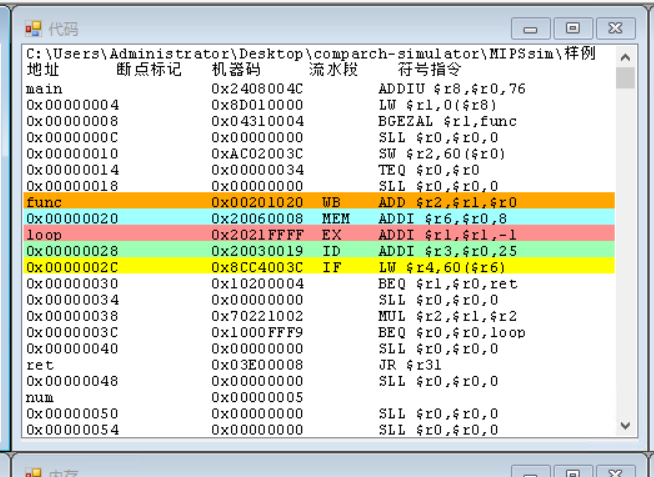
\includegraphics[width=0.9\textwidth]{images/t13seg.png}
		\caption{各段正在处理的指令}
		\label{fig:t13seg}
	\end{subfigure}
	\begin{subfigure}[b]{0.4\textwidth}
		\centering
		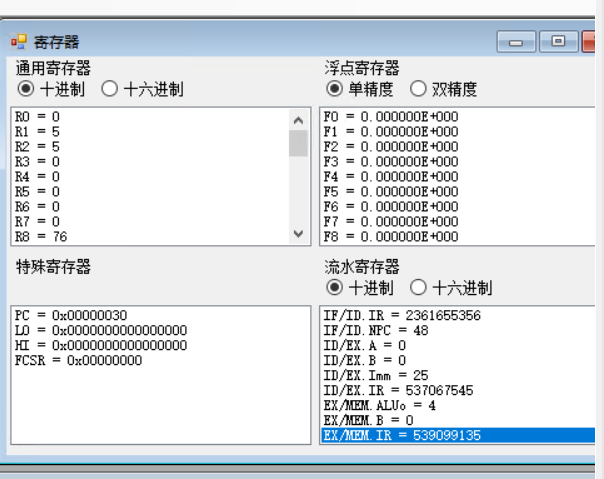
\includegraphics[width=0.9\textwidth]{images/t13reg1.png}
		\caption{各流水寄存器中的内容(1)}
		\label{fig:t13reg}
	\end{subfigure}
	\begin{subfigure}[b]{0.4\textwidth}
		\centering
		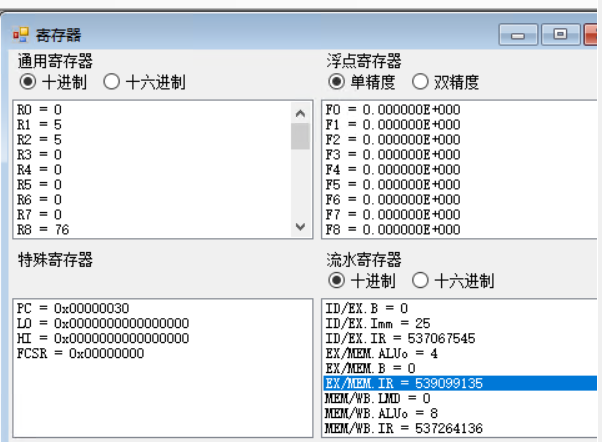
\includegraphics[width=0.9\textwidth]{images/t13reg2.png}
		\caption{各流水寄存器中的内容(2)}
		\label{fig:t13reg}
	\end{subfigure}
	\begin{subfigure}[b]{0.4\textwidth}
		\centering
		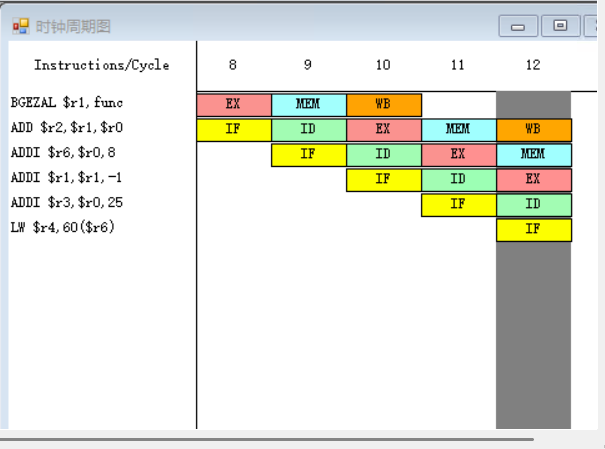
\includegraphics[width=0.9\textwidth]{images/t13clock.png}
		\caption{时钟周期图}
		\label{fig:t13clock}
	\end{subfigure}
\end{figure}

加载\texttt{structure\_hz.s},执行该程序,总周期数52个,结构停顿周期数41个,占总执行周期数的78.85\%
如图~\ref{fig:structhz}。将浮点加法器改为4个,可以发现总周期
数变为19个,结构停顿周期数变为8个,占总执行周期数的比例变为42.11\%。如图~\ref{fig:structhz4}。
\begin{figure}[htb]
	\centering
	\begin{subfigure}[b]{0.4\textwidth}
		\centering
		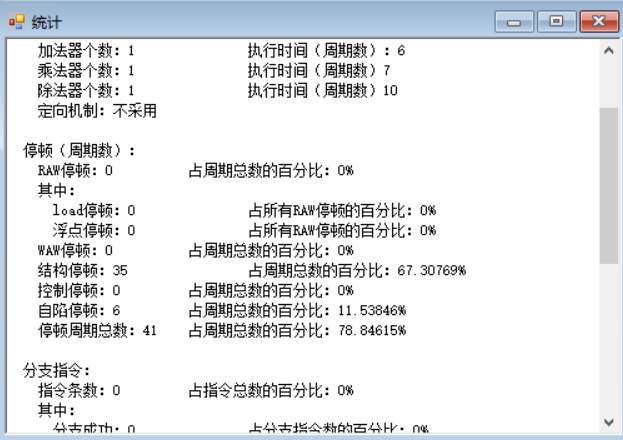
\includegraphics[width=0.9\textwidth]{images/structhz.png}
		\caption{结构停顿周期数为41个}
		\label{fig:structhz}
	\end{subfigure}
	\begin{subfigure}[b]{0.4\textwidth}
		\centering
		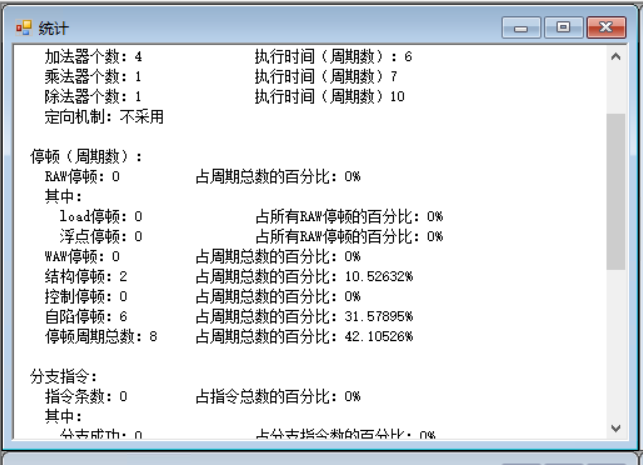
\includegraphics[width=0.9\textwidth]{images/structhz4.png}
		\caption{结构停顿周期数为8个}
		\label{fig:structhz4}
	\end{subfigure}
\end{figure}

\subsubsection{实验结论}

由以上实验结果可知,发生冲突时,流水线会出现停顿从而降低CPU的性能,增加时钟周期数。
结构停顿周期数的减少,可以提高CPU的性能。

为了解决这一问题,可以在流水线处理机中设置足够多的相互独立的指令寄存器和数据寄存器,
或者改变程序的设计,尽量减少停顿的发生。

\subsection{观察数据冲突并用定向技术来减少停顿}

关闭定向技术,执行\texttt{data\_hz.s}程序,执行结果
如图~\ref{fig:nofwd}。
\begin{figure}[htb]
	\centering
	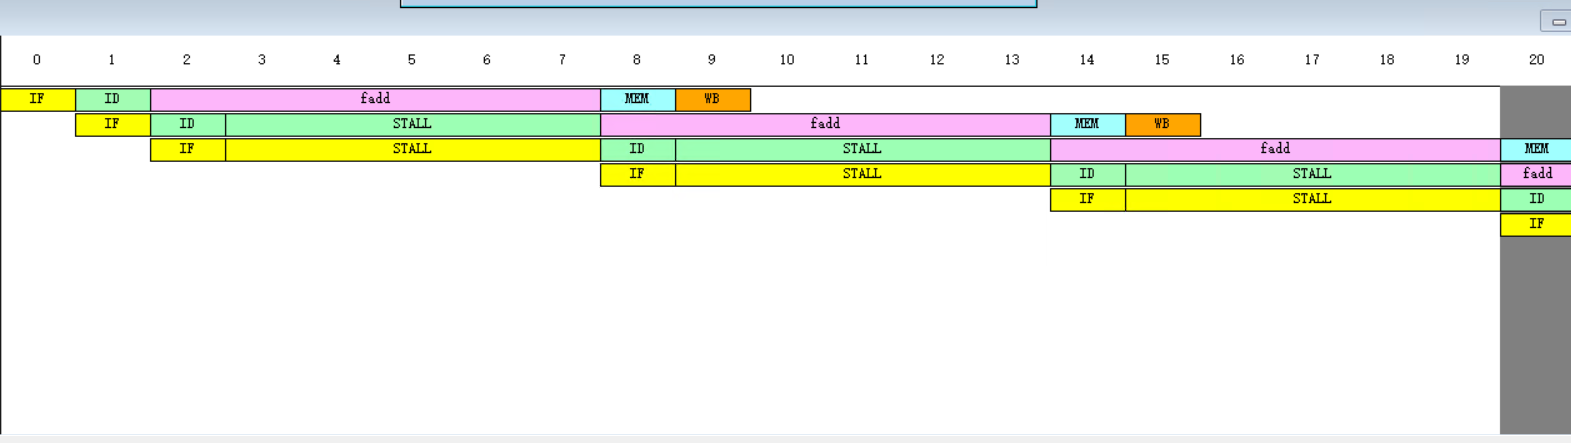
\includegraphics[width=0.9\textwidth]{images/nofwd.png}
	\caption{关闭定向技术}
	\label{fig:nofwd}
\end{figure}

可以观察到在第4,6,7,9,10,13,14,17,18,20,21,25,26,28,29,32,33,36,
 37,39,40,44,45,47,48,51,52,55,56,58,59 时钟周期发生RAW冲突。

启动定向技术,执行\texttt{data\_hz.s}程序,执行结果
如图~\ref{fig:withfwd}。
\begin{figure}[htb]
	\centering
	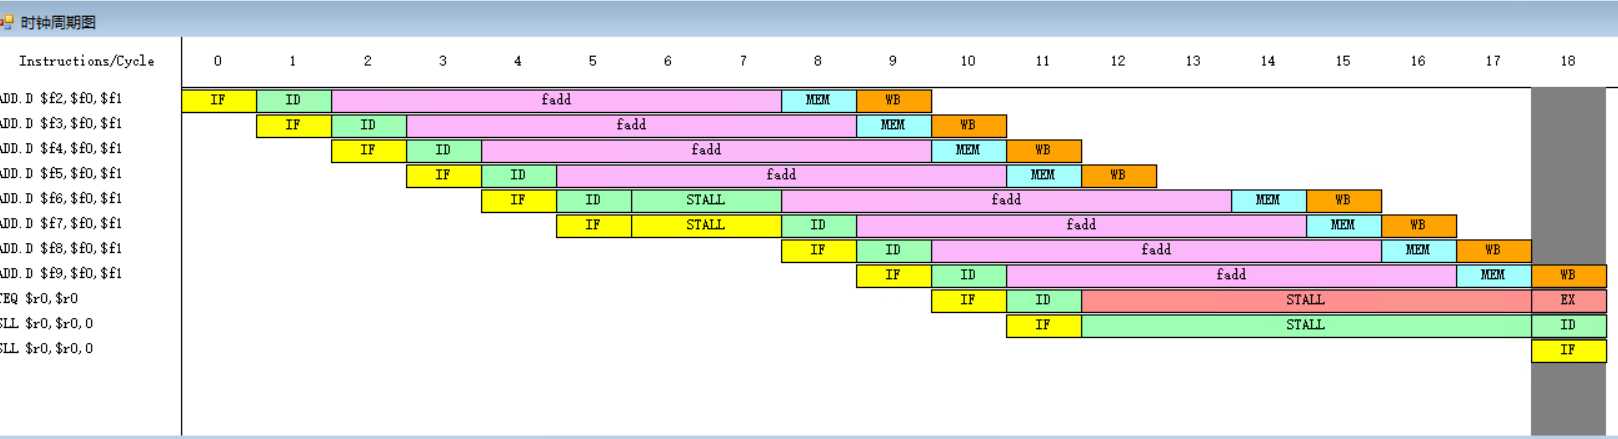
\includegraphics[width=0.9\textwidth]{images/fwd.png}
	\caption{启动定向技术}
	\label{fig:withfwd}
\end{figure}
在第 5,10,13,18,22,25,30,34,37 时钟周期发生了RAW冲突,相比之下大大减少

对比是否启用定向技术,可以发现启用定向技术后,结构停顿周期数减少了很多,如图~\ref{fig:cmpfwd}。
\begin{figure}[htb]
	\centering
	\begin{subfigure}[b]{0.4\textwidth}
		\centering
		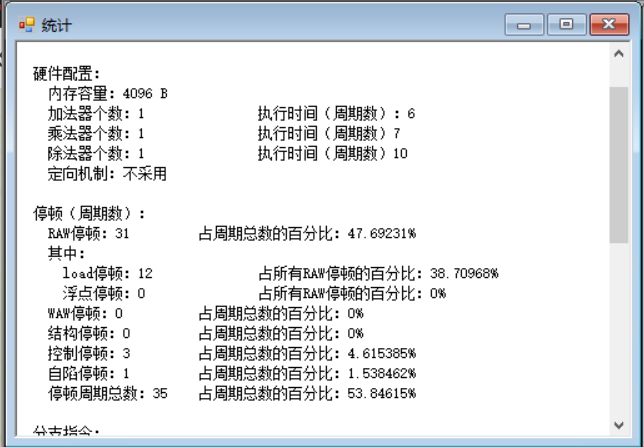
\includegraphics[width=0.9\textwidth]{images/nofwdsts.png}
		\caption{关闭定向技术}
		\label{fig:nofwdsts}
	\end{subfigure}
	\begin{subfigure}[b]{0.4\textwidth}
		\centering
		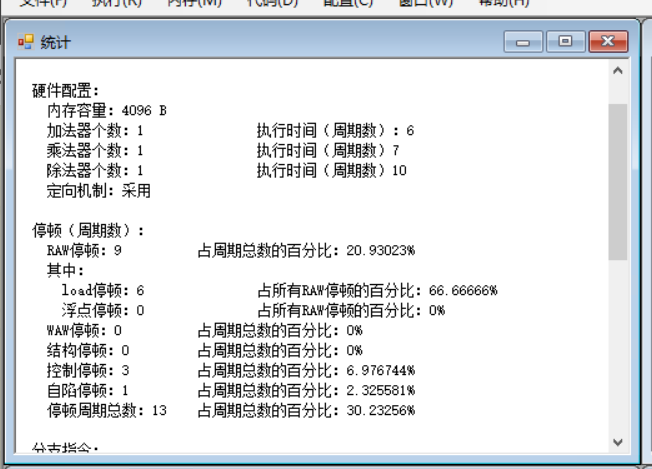
\includegraphics[width=0.9\textwidth]{images/withfwdsts.png}
		\caption{启动定向技术}
		\label{fig:withfwdsts}
	\end{subfigure}
\end{figure}

可以发现数据冲突引起的停顿周期数为9,程序的总时钟周期数为43,停顿时钟周期数占总执行周期数的百分比为20.93023\%,
采用定向技术后的性能是原来的1.51倍。

\section{补充实验}

\subsection{实验题目}

编写程序。在流水线 CPU 中,立方和公式的两种计算方法应该如何安排指令使得结构停顿占周期总数的百分比最小?
两种方法的性能之比?立方和的两种公式如\eqref{eqn:cubicsum}
\begin{equation}
	\label{eqn:cubicsum}
	\begin{aligned}
		& a^3+b^3 \\
		& (a+b)(a^2-b^2+ab) \\
	\end{aligned}
\end{equation}
其中$a$、$b$的初始值存放在\texttt{R1 R2}寄存器中,计算结果存放在\texttt{R3}寄存器中。从\texttt{R4}开始使用寄存器,数量不限。

\subsection{代码实现}

为了最大限度地减少代码中的相关,我按照以下原则来实现代码:
\begin{itemize}
	\item 前后两条指令读写的寄存器尽量不相同;
	\item 访存的指令尽量相邻;
	\item 尽量减少计算中的依赖关系;
\end{itemize}
然后根据结果再实际调整代码,使得停顿占周期总数的百分比最小。

\subsection{$a^3+b^3$}

计算$a^3+b^3$,首先从内存中加载操作数,然后
计算$a^2$,然后计算$b^2$,最后分别计算$a^3$和$b^3$再求和,
最后将$a^3+b^3$的结果存放在\texttt{R3}寄存器中。
这样做总的停顿次数为$5$次。实现如代码~\ref*{code:first}
\begin{listing}[htb]
	\caption{计算$a^3+b^3$}
	\label{code:first}
	\inputminted{nasm}{../code/good/mul.s}
\end{listing}


\subsection{$(a+b)(a^2-b^2+ab)$}

计算$(a+b)(a^2-b^2+ab)$,首先从内存中加载操作数,然后分别计算
$a^2$、$b^2$和$ab$,然后计算$a^2-b^2+ab$,最后计算$(a+b)(a^2-b^2+ab)$,
最后将$(a+b)(a^2-b^2+ab)$的结果存放在\texttt{R3}寄存器中。
这样做总的停顿次数为$6$次。实现如代码~\ref*{code:second}
\begin{listing}[htb]
	\caption{计算$(a+b)(a^2-b^2+ab)$}
	\label{code:second}
	\inputminted{nasm}{../code/good/mul2.s}
\end{listing}

\subsection{运行结果和计算}

两段程序的运行结果如图~\ref*{fig:res}。前者的停顿周期数为5,后者的停顿周期数为6。
运行效率之比为:
\begin{equation}
	\frac{CPI_1}{CPI_2}\approx1.14
\end{equation}

\begin{figure}[H]
	\centering
	\caption{计算$a^3+b^3$和$(a+b)(a^2-b^2+ab)$的运行结果}
	\label{fig:res}
	\begin{subfigure}[b]{0.4\textwidth}
		\centering
		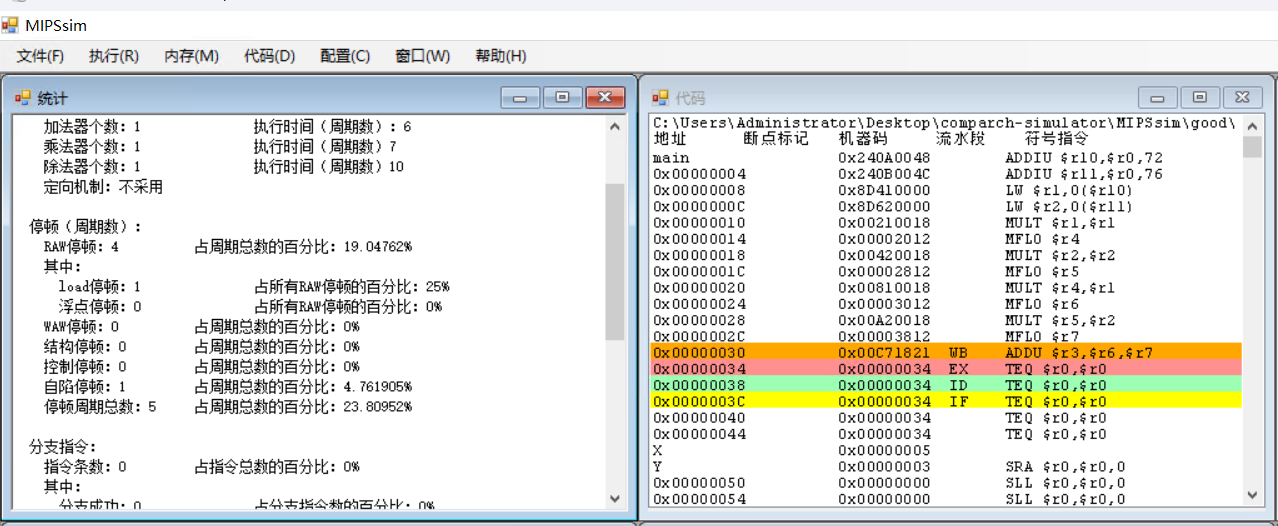
\includegraphics[width=0.9\textwidth]{images/mul.png}
		\caption{计算$a^3+b^3$}
	\end{subfigure}
	\begin{subfigure}[b]{0.4\textwidth}
		\centering
		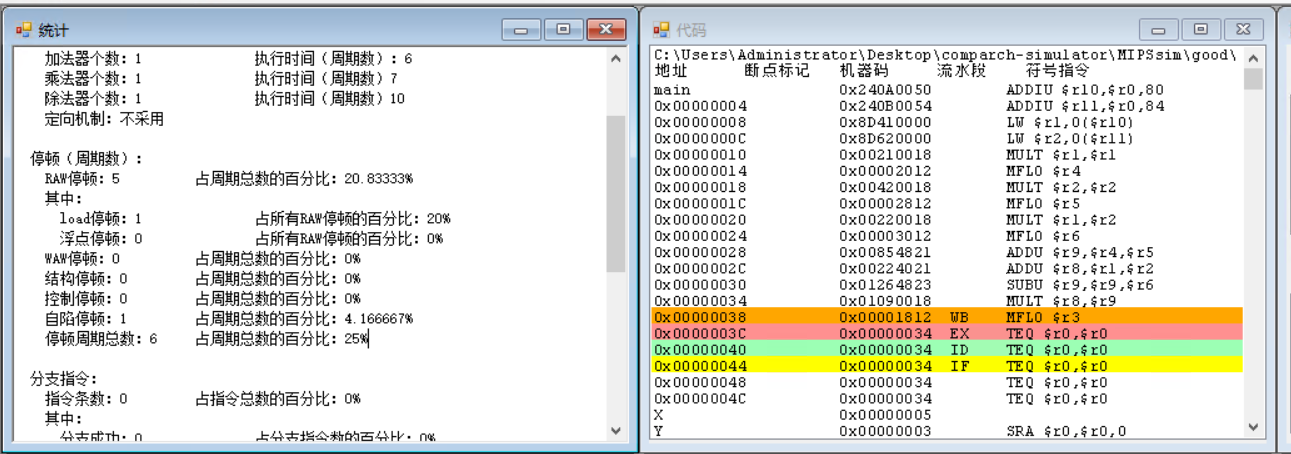
\includegraphics[width=0.9\textwidth]{images/mul2.png}
		\caption{计算$(a+b)(a^2-b^2+ab)$}
	\end{subfigure}
\end{figure}


\clearpage

\section{实验总结}

在此次实验中,我加深了对计算机流水线基本概念的理解,理解了MIPS结构如何用5段流水线来实现,
理解了各段的功能和基本操作,加深了对数据冲突、结构冲突的理解,理解了这两类冲突对CPU性能的影响。
并且进一步理解了解决数据冲突的方法,掌握了如何应用定向技术来减少数据冲突引起的停顿。
并且实际编写了计算立方和的程序来对比不同计算方法产生的误差。

\end{spacing}

\end{document}